\documentclass[a4paper,12pt]{article} 
\usepackage[T2A]{fontenc}			
\usepackage[utf8]{inputenc}			
\usepackage[english,russian]{babel}	
\usepackage{amsmath,amsfonts,amssymb,amsthm,mathrsfs,mathtools} 
\usepackage{cancel}
\usepackage{multirow}
\usepackage[colorlinks, linkcolor = blue]{hyperref}
\usepackage{upgreek}\usepackage[left=2cm,right=2cm,top=2cm,bottom=3cm,bindingoffset=0cm]{geometry}
\usepackage{graphicx}
\usepackage{xcolor}
\usepackage{wrapfig}
\author{Дорогинин Д.В.\\
Группа Б02-825}
\title{4.3.1. Изучение дифракции света}
\date{}
\begin{document}
\maketitle
\textbf{Цель работы}: исследовать являения дифракции Френеля и Фраунгофера на щели, изучить влияние дифракции на разрешающую способность оптических инструментов.


\textbf{В работе используются}: оптическая скамья, ртутная лампа, монохроматор, щели с регулируемой шириной, рамка с вертикальной нитью, двойная щель, микроскоп на поперечных салазках с микрометрическим винтом, зрительная труба.
\section*{Описание работы}
\subsection*{А. Дифракция Френеля}
\begin{figure}[h]
\includegraphics[scale=0.7]{0.png}
\centering
\caption{Схема установки 1.}
\end{figure}
Схема установки представлена на Рис. 1. Световые лучи освещают щель $S_2$ и испытывают на ней дифракцию. Дифракционная картина рассматривается с помощью микроскопа М, сфокусированного на некоторую плоскость наблюдения П. Щель $S_2$ освещается параллельным пучком монохроматического света с помощью коллиматора, образованного объективом $O_1$ и щелью $S_1$, находящейся в его фокусе. На $S_1$ сфокусированно изображение спектральной линии, выделенной из спектра ртутной лампы Л при помощи монохроматор $C$, в котором используется призма прямого зрения. \\
Распределение интенсивности света в плоскости П рассчитаем с помощью зон Френеля. При освещении $S_2$ параллельным пучком лучей (плоская зона) зоны Френеля представляют собой плоскости, параллельные краям щели. Результирующая амплитуда в точке наблюдения определеяется суперпозицией колебаний от тех зон Френеля, которые не перекрыты створками щели. Графическое определение результирующей амплитуды производится с помощью векторной диаграммы -- спирали Корню. Суммарная ширина $m$ зон Френеля $z_m$ определяется соотношение
\begin{equation}
z_m = \sqrt{am\lambda},
\end{equation}
где $a$ -- расстояние от щели до плоскости П. Вид наблюдаемой картины определяется \textit{числом Френеля} $\Phi$:
$$
\Phi^2 = \dfrac{D}{\sqrt{a\lambda}}
$$
-- число зон Френеля, которые укладываются в ширине щели $D$. $p = \frac{1}{\Phi^2}$ называется \textit{волновым параметром}. Дифракционной картины нет, когда П совпадает с плоскостью щели. При малом удалении от щели $\Phi \gg 1$ и картина наблюдается в узкой убласти на границе света и тени у краёв экрана. При последующих удалениях две группы дифракционных полос перемещаются независимо и каждая образует картину дифракции Френеля на экране. Распределение интенсивности может быть найдено с помощью спирали Корню. При дальнейшем увеличении $a$ две системы полос сближаются и накладываются друг на друга, распределение интенсивности определяется числом зон Френеля в полуширине щели. Если их $m$, то будет набюдаться $m-1$ тёмная полоса.
\subsection*{Б. Дифракция Фраунгофера на щели}
\begin{wrapfigure}{r}{0.5\textwidth}
  \begin{center}
    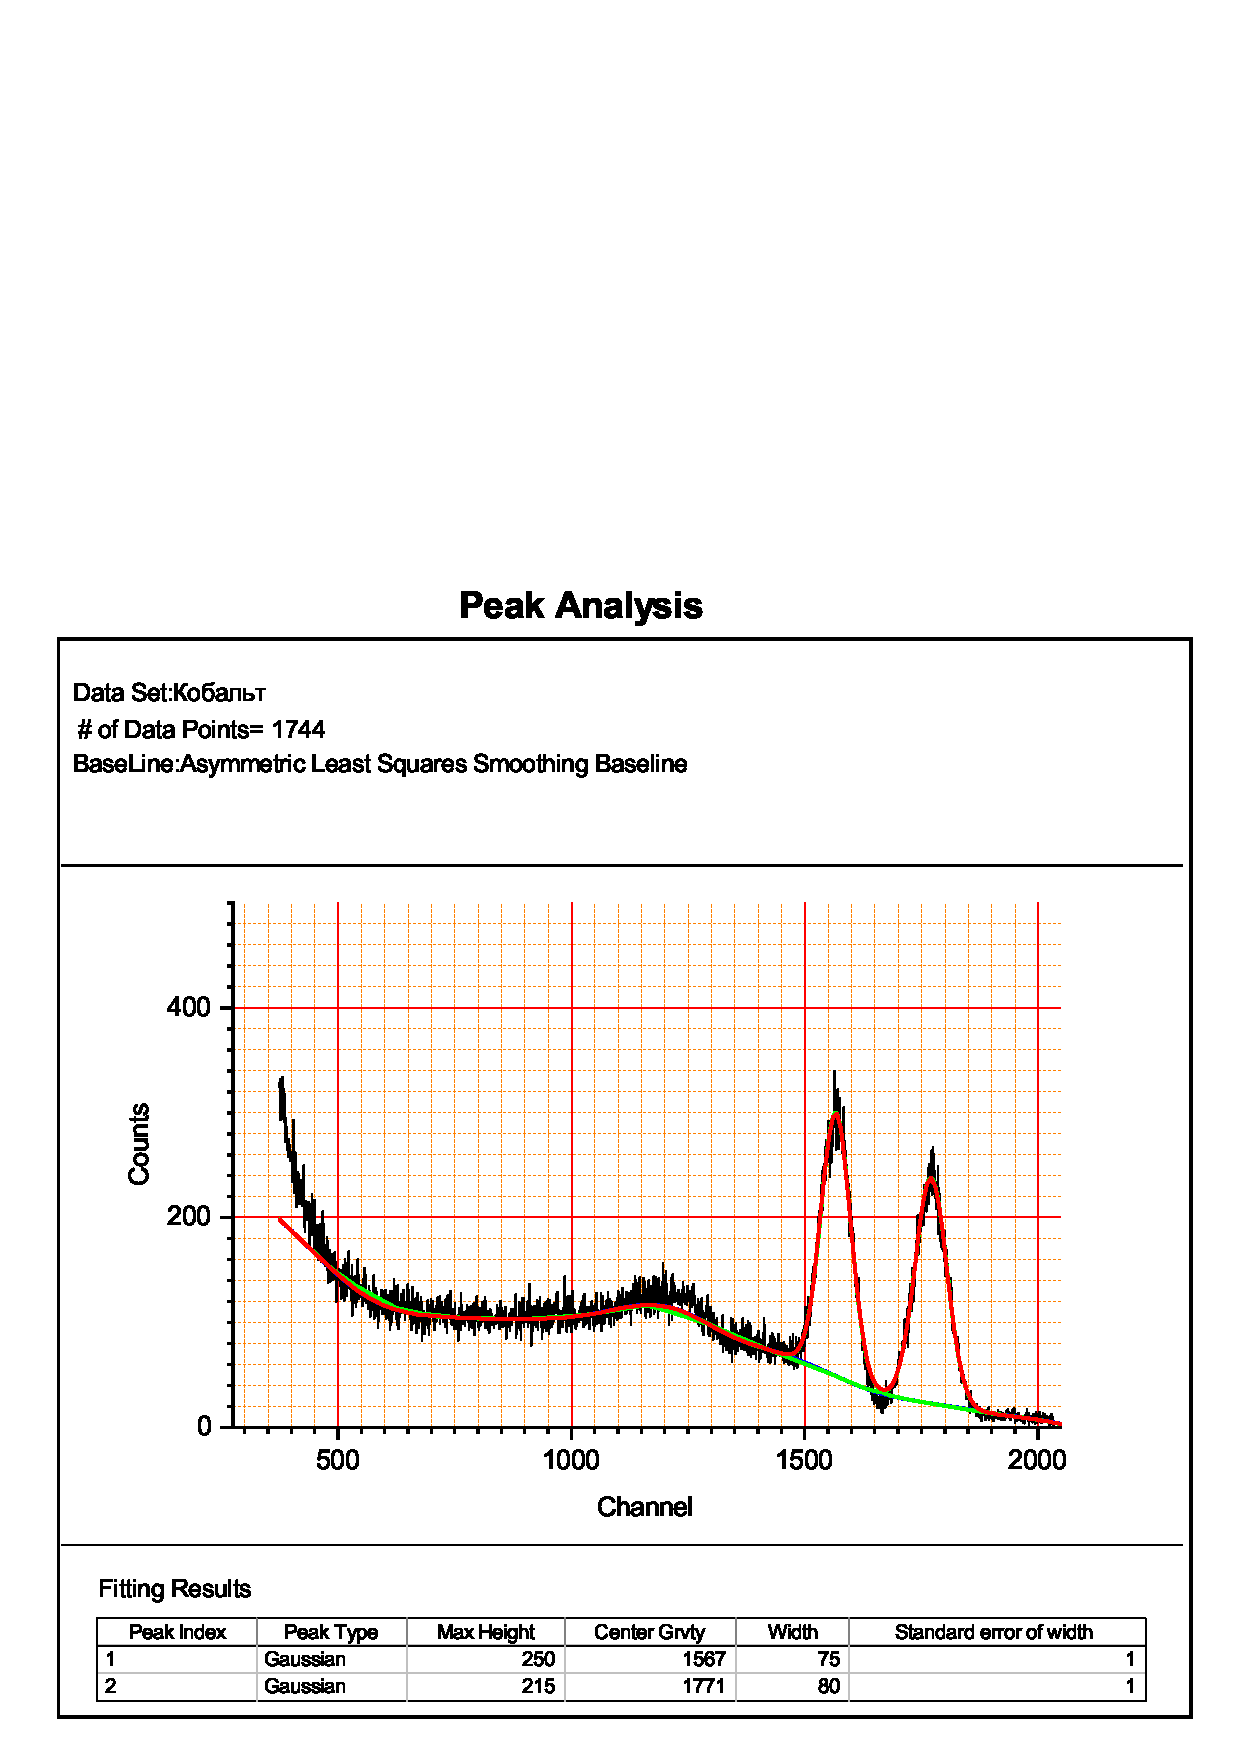
\includegraphics[width = 0.4\textwidth]{2.png}
  \end{center}
  \caption{Построение зон Френеля}
\end{wrapfigure}
Для выкладок ниже нам потребуется знать \textit{принцип Гюйгенса-Френеля}. Он формулируется следующим образом:\\
\textit{Каждый элемент волнового фронта можно рассматривать как центр  вторичного возмущения, порождающего вторичные сферические волны, а результирующее световое поле  в каждой точке пространства будет определяться интерференцией этих волн.}\\
Теперь рассмотрим первое применение этого принципа, получившее название \textit{метод зон Френеля}

\begin{wrapfigure}{r}{0.3\textwidth}
  \begin{center}
    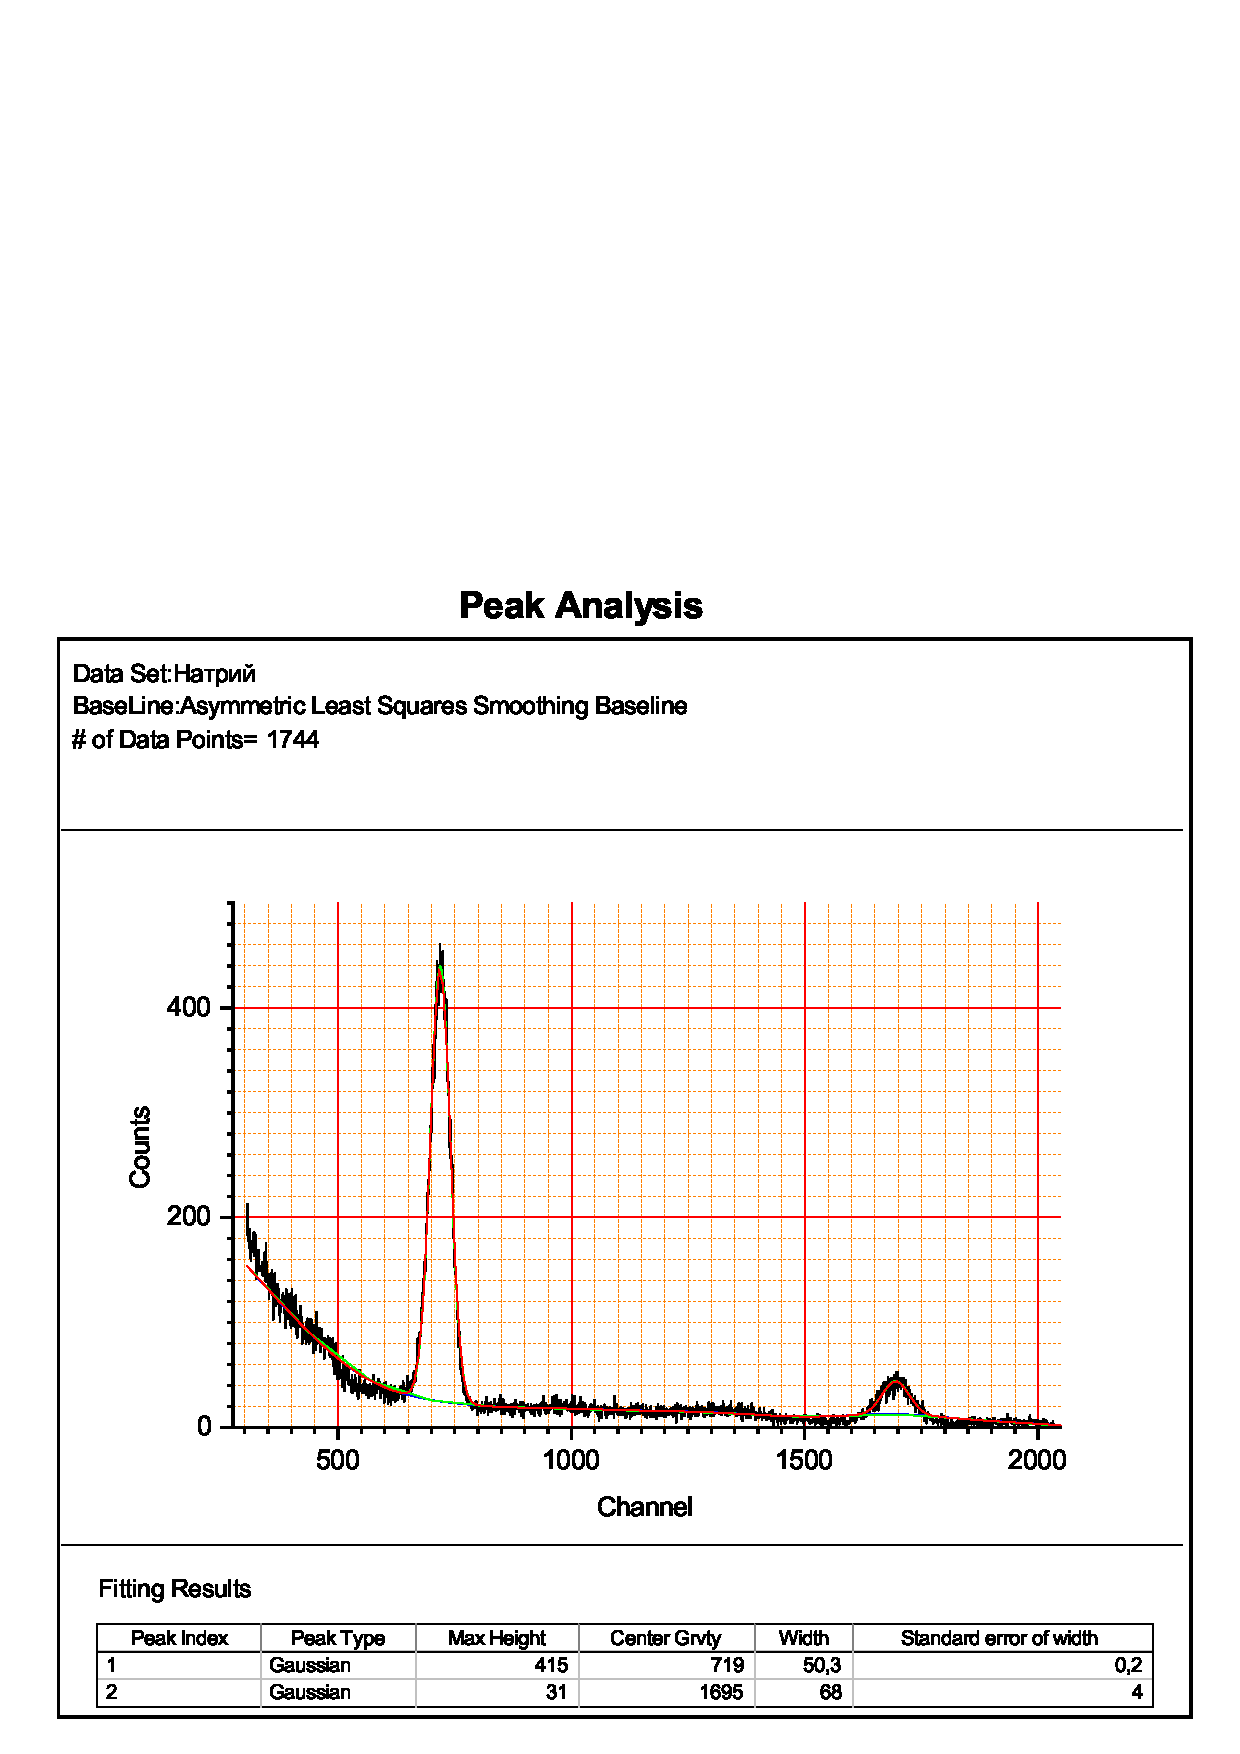
\includegraphics[width = 0.3\textwidth]{1.png}
  \end{center}
  \caption{К фазовым соотношениям при дифракции Фраунгофера}
  \vspace{+30pt}
\end{wrapfigure}

Для этого рассмотрим действие световой волны действующей из точки $A$ в какой-то точке $B$.
В этом случае можно, взяв точку $M_0$ в качестве центра (см. рис. 1), построить ряд концентрических сфер, радиусы которых начинаются с $b$ и увеличиваются каждый раз на половину длины волны $\frac{\lambda}{2}$. При пересечении с плоским фронтом волны $F$ эти сферы дадут концентрические окружности. Таким образом, на фронте волны появятся кольцевые зоны (зоны Френеля) с радиусами $r_1, r_2$ и т. д.

Из геометрических соображений посчитав, можно получить, что 
\begin{equation}
r_i = i \sqrt{a \lambda}
\end{equation}

Картина дифракции упрощается, когда ширина щели становится значительно меньше ширины первой зоны Френеля, т.е. если 
\begin{equation}
D \ll\sqrt{a \lambda} 
\end{equation}	
Это условие всегда выполняется при достаточно большом $a$. В этом случае говорят, что \textit{дифракция Фраунгофера}. Дифракционную картину в этом случае называются \textit{дифракцией Фраунгофера}. При выполнении пункта $(2)$ у нас упрощаются фазовые соотношения, что поясняет рис. 2, в итоге с хорошим приближением можно считать, что разность хода между крайними лучами, приходящими от щели в точке наблюдения $P$, с хорошим приближением равна 
\begin{equation}
\Delta = r_2 - r_1 \approx D \sin \theta \approx D \cdot \theta
\end{equation}
Здесь предполагается, что $\theta$ достаточно мал.
Дифракцию Фраунгофера можно наблюдать на установке Рис. 1, но для удобства к подобной установке добавляется объектив $O_2$.

\begin{figure}[h]
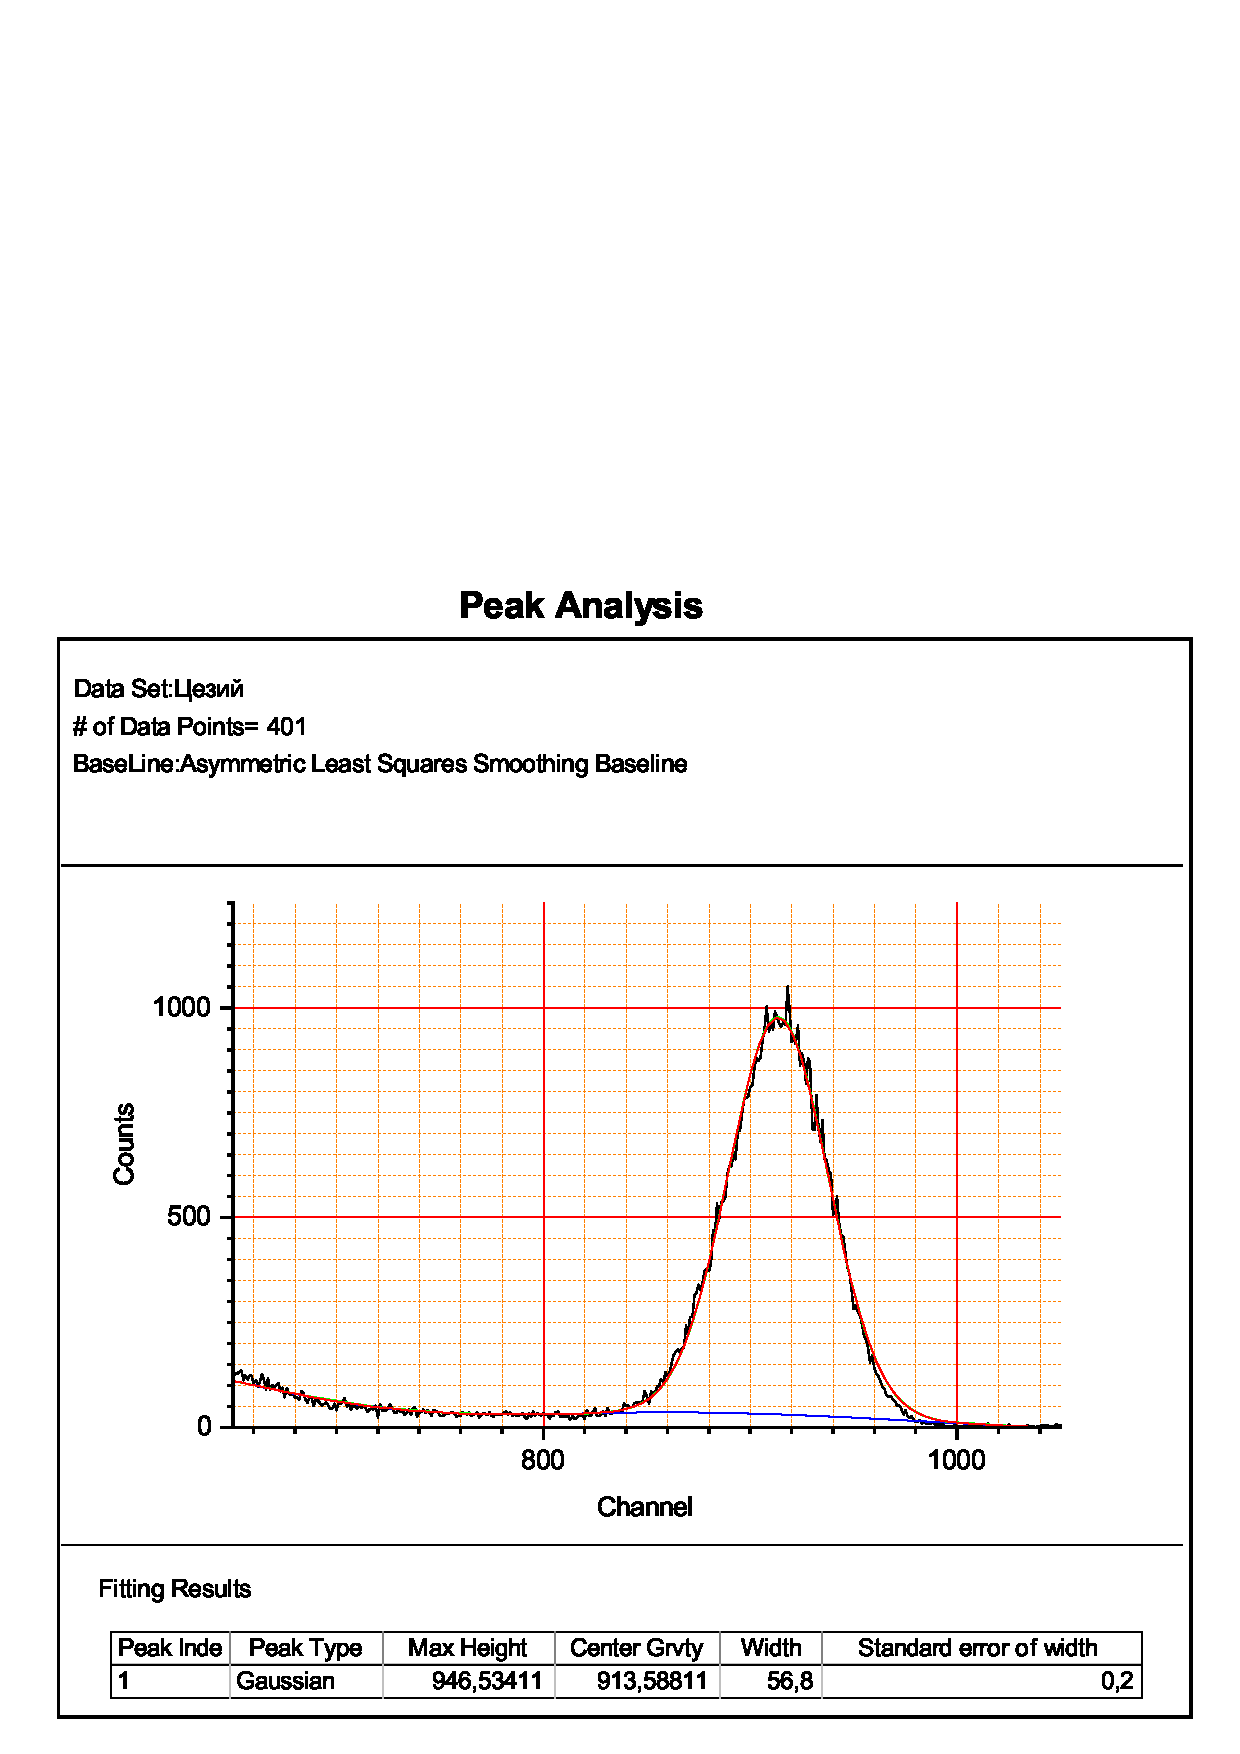
\includegraphics[width = 0.7\textwidth]{3.png}
\centering
\caption{Схема установки 2.}
\end{figure}
Дифракционная картина здесь наблюдается в фокальной плоскости объектива $O_2$. Каждому значению $\theta$ соответствует в этой плоскости точка, отстоящая от оптической оси на расстоянии 
\begin{equation}
X = f_2 \tan \theta \approx f_2 \theta.
\end{equation}
Объектив не вносит разности хода между интерферирующими лучам, поэтому в его фокальной плоскости наблюдается неискажённая дифракционная картина. При $\theta = 0$ разность хода между лучами нулевая, поэтому в центре поля зрения дифракционный максимум. Первый минимум соответствует $\theta_1$ такому, что в точке наблюдения разность хода пробегаем все значения от 0 до $2\pi$. Аналогично рассуждая, для $m$-й полосы
\begin{equation}
\theta_m = \frac{m \lambda}{D}
\end{equation}
Расстояние $X_m$ тёмной полосы от оптической оси из (5) и (6)
\begin{equation}
X_m = f_2m\frac{\lambda}{D}
\end{equation}
\subsection*{В. Дифракция Фраунгофера для двух щелей}
Для наблюдения дифракции Фраунгофера на двух щелях $S_2$ заменим экраном Э с двумя щелями. При этом для оценки влияния ширины входной щели на чёткость вместо $S_1$ поставим щель с микрометрическим винтом.
\begin{figure}[h]
\includegraphics[width = 0.7\textwidth]{4.png}
\centering
\caption{Схема установки 3.}
\end{figure}
Два дифракционных изображения входной щели, одно из которых образовано лучами, прошедшими через левую, а другое -- через правую щели, накладываются друг на друга.
Если входная щель достаточно узка, то дифракционная картина в плоскости П подобна той, что получалась при дифракции на одной щели, однако вся картинка испещерена рядом дополнительных узких полос, наличие которых объясняется суперпозицией световых волн через разные щели. Светлая интерфереционная полоса наблюдается в случаях, когда разность хода равна целому числу длин волн. Таким образом, угловая координата максимума порядка $m$ равна
\begin{equation}
\theta_m = \dfrac{m \lambda}{d},
\end{equation}
где $d$ -- расстояние между щелями. Отсюда расстояние между соседними интерфереционными полосами в плоскости П равно
\begin{equation}
\delta x = f_2 \dfrac{\lambda}{d}
\end{equation}
Число интерференционных полос укладывающихся в области центрального максимума равна отношению ширины главного максимума $\frac{2\lambda f_2}{D}$ к расстоянию между соседними полосами:
\begin{equation}
n = \dfrac{2\lambda f_2}{D} \dfrac{1}{\delta f}= \dfrac{2d}{D}.
\end{equation}
При дифракции света на двух щелях чёткая система интерференционных полос наблюдается только при достаточно узкой ширине входной щели $S$. При увеличении ширины картинка пропадает и появляется вновь, но полосы при этом сильно размыты и видны плохо.
\subsection*{Г. Влияние дифракции на разрешающую способность оптического инструмента}
\begin{figure}[h]
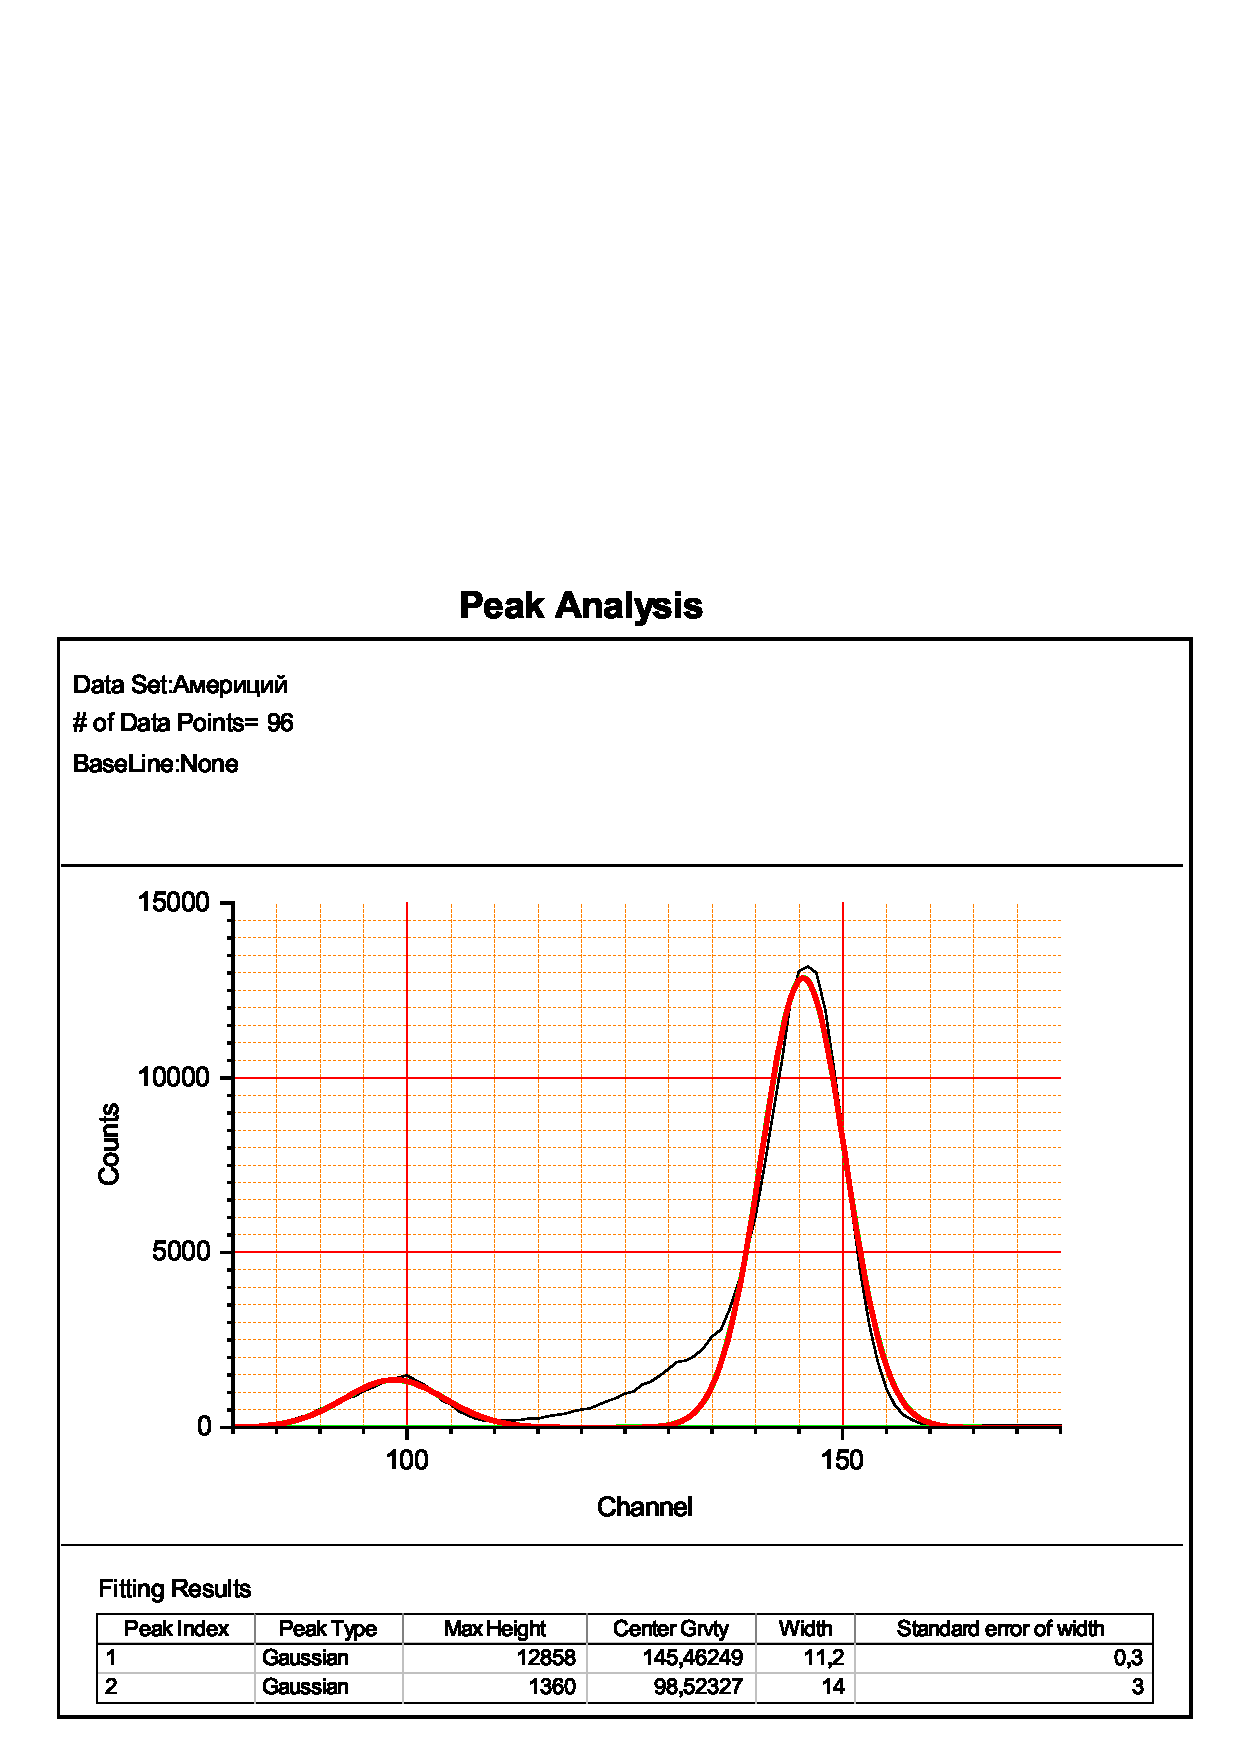
\includegraphics[width = 0.8\textwidth]{5.png}
\centering
\caption{Схема установки 4.}
\end{figure}
В отсутствие щели $S_2$ линзы $O_1$ и $O_2$ создают на плоскости П изоюражение щели $S_1$ и это изображение рассматриваются микроскопом М. Таким образом, установку можно рассматривать как оптический инструмент, предназначенные для получения изображения предмета. Если перед $O_2$ расположить $S_2$, то изображение объекта будет искажено из-за дифракции. Чем меньше ширина щели, тем сильнее искажение. Качественной характеристикой этого искажения может служить $\varphi_{min}$ --- минимальное угловое расстояние между объектами (источниками), которые всё ещё воспринимаются как раздельные. Поместим вместо $S_1$ экран Э с двумя щелями с расстоянием $d$. Тогда на $S_2$ будут падать два пучка света с углом
\begin{equation}
\varphi = \dfrac{d}{f_1}
\end{equation}
Из геометрии расстояние $l$ между изображениями щелей в плоскости П равно 
\begin{equation}
l = \varphi f_2 = d \dfrac{f_2}{f_1}.
\end{equation}
Ширина $\Delta \varphi$ определяется дифракцией на $S_2$. Условия, при которых изображения различимы разные для разных наблюдателей, поэтому используют \textit{критерий Рэлея} -- \textit{максимум одного дифракционного пятна должен совпадать с минимумом другого}. В наших условиях это значит, что угловая полуширина $\frac{\lambda}{D}$ равна угловому расстоянию $\frac{l}{f_2}$.
\newpage
1
\newpage
2
\newpage
\section*{Ход работы}
\subsection*{А. Дифракция Френеля}
В ходе всей работы $\lambda = 579.07 \text{ нм}$.
Положение микроскопа, при котором на фоне щели видна одна полоса -- $x_0 = 55.4 \pm 0.1 \text{ см}$, в качестве погрешности выбираем половину цену деления линейки. Измерим ширину щели микрометрическим винтом и с помощью поперечных салазок микроскопа:
$$
\begin{array}{l}
D_{\text{винт}} = 335\pm 5 \text{ мкм},\\
D_{\text{микро}} = 320\pm 10 \text{ мкм},
\end{array}
$$
В качестве погрешности берём половину цены деления шкал соответствующих приборов.\\
Зависимость количества полос от расстояния до экрана представлена в Таблице 1. Здесь $a_n$ -- смещение от положения $x_0$, $z_n$ находится из формулы (1).
\begin{table}[h!]
\begin{tabular}{|c|c|c|c|c|c|}
\hline
$m$ & $x$, см&  $\sigma_x$, см  &  $a_n$, см & $2 z_n$, мкм & $\sigma_{2z_n}$, мкм \\
\hline
1 & 52,6 & 0,1 & 2,8 & 255 & 5\\
2 & 53,5 & 0,1 & 1,9 & 297 & 8\\
3 & 54,1 & 0,1 & 1,3 & 301 & 12\\
4 & 54,4 & 0,1 & 1,0 & 304 & 15\\
5 & 54,5 & 0,1 & 0,9 & 323 & 18\\
\hline
\end{tabular}
\centering
\caption{Зависимость $z_n = f(a_n)$.}
\end{table}\\
Погрешность $2z_m$ считается по формуле
$$
\varepsilon_{z_n} = \dfrac{1}{2} \varepsilon_{a_n} \Rightarrow \sigma_{2z_n}= \dfrac{z_n}{2} \varepsilon_{a_n}.
$$
Усредним $2z_n$ и получим $D$ -- ширину щели. Погрешность для неё считается по формуле 
$$
\sigma_D = \sqrt{\sigma_{\bar{D}}^2 + \tilde{\sigma}_{D}^2},
$$
где $\sigma_{\bar{D}}$ -- погрешность $D$, 
$$
\tilde{\sigma}_{D} = \dfrac{1}{\sqrt{n(n-1)}} \cdot \sqrt{\sum\limits_{i = 1}^n\left(2z_i - D\right)^2}.
$$
Итоговое значение 
\begin{center}
\fbox{$D = 296 \pm 16 \text{ мкм}$}
\end{center}
\subsection*{Б. Дифракция Фраунгофера на щели}
Фокусные расстояния линз $F_1 = 12.8 \text{ см}$, $F_2 = 11.5 \text{ см}$. Ширина щели $D = 400 \pm 5 \text{ мкм}$ (погрешность -- половина цены деления микрометрического винта).\\
Измеренные координаты $X_m$ минимумов представлены в Таблице 2.
\newpage
\begin{table}[]
\begin{tabular}{|c|c|c|c|c|c|c|c|c|}
\hline
$m$      & 1    & 2    & 3   & 4    & -1   & -2   & -3  & -4   \\ \hline
$X_m$, мм & 0.16 & 0.34 & 0.50 & 0.66 & 0.14 & 0.34 & 0.50 & 0.66 \\ \hline
$\sigma_{X_m}$, мм & 0.02 & 0.02 & 0.02 & 0.02 & 0.02 & 0.02 & 0.02 & 0.02 \\ \hline
$D$, мкм      & 420  & 390  & 400 & 404  & 480  & 400  & 400 & 404  \\ \hline
$\sigma_D$, мкм  & 50   & 20   & 16  & 12   & 70   & 20   & 16  & 12   \\ \hline
\end{tabular}
\centering
\caption{Зависимость $X_m = f(m)$.}
\end{table}
$D$ здесь считается по формуле (7), погрешность для $D$ 
$$
\sigma_D = \sqrt{\left(\dfrac{\partial \left(f_2 m \frac{\lambda}{X_m}\right)}{\partial X_m}\right)^2 \cdot \sigma^2_{X_m}} = \dfrac{f_2m \lambda}{X_m^2} \cdot \sigma_{X_m} = \dfrac{D}{X_m} \cdot \sigma_{X_m}.
$$ 
Аналогично предыдущему пункту расчитаем среднее $D$:
\begin{center}
\fbox{$D = 410 \pm 30 \text{ мкм}$}
\end{center}
\begin{figure}[h]
\includegraphics[scale=0.7]{10.png}
\centering
\caption{График зависимости $X_m = f(m)$.}
\end{figure}
Зависимость $X_m = f(m)$ представлена на Рис. 7. По наклону графика $X_m = f(m)$ определим $\Delta X$ -- расстояние между соседними минимумами. Приближаем прямой $y = kx$, получили 
$$
\Delta X = 0.1657 \pm 0.0013 \text{ мм}.
$$ 
\subsection*{В. Дифракция Фраунгофера для двух щелей}
Расстояние между тёмными полосами, отстающими друг от друга на максимальное расстояние: $\Delta X = 0.72 \pm 0.01 \text{  мкм}$, между ними $n_{\text{эксп}} = 11 \pm 1$ светлых промежутков. Тогда $\delta x = \frac{\Delta X}{n} = 65 \pm 7 \text{ мкм}$. Погрешность определяется по формуле:
$$
\sigma_{\delta x} = \sqrt{\left(\dfrac{\partial \left(\frac{\Delta X}{n}\right)}{\partial \Delta X}\right)^2 \sigma^2_{\Delta X} + \left(\dfrac{\partial \left(\frac{\Delta X}{n}\right)}{\partial n}\right)^2 \sigma^2_{n}} =\sqrt{\dfrac{\sigma^2_{\Delta X}}{n^2} + \dfrac{\Delta X^2 \sigma^2_{n}}{n^4}}.
$$
Из формулы (9) получаем $d = 1.02 \pm 0.04 \text{ мм}$. Погрешность $d$ определяется по формуле:
$$
\sigma_d = \sqrt{ \left(\frac{\partial \left(\frac{f_2\lambda}{\delta x}\right)}{\partial \delta x}\right)^2 \sigma^2_{\delta x}} = \dfrac{f_2 \lambda}{\delta x^2} \sigma_{\delta x}.
$$
Из измерений $d = 1.00 \pm 0.01 \text{ мм}$, $D = 0.20 \pm 0.01 \text{ мм}$ (погрешность -- половина цены деления шкалы микроскопа), откуда из формулы (10) $n_{\text{теор}} = 10 \pm 1$. Погрешность для $n_{\text{теор}}$ находим по формуле
$$
\sigma_n = \sqrt{\left( \frac{\partial \left( \frac{2d}{D}\right)}{\partial d} \right)^2 \sigma_d^2 + \left( \dfrac{\left(\frac{2d}{D}\right)}{D}\right)^2 \sigma_D^2} = \sqrt{\dfrac{4 \sigma_d^2}{D^2} + \dfrac{4d^2 \sigma_D^2}{D^4}}.
$$
Интерфереционные полосы исчезают при $b_0 = 70 \pm 10 \text{ мкм}$ (погрешность -- половина цены деления шкалы микроскопа). Из формулы 
\begin{equation}
\dfrac{b}{f_1} = \dfrac{\lambda}{d}
\end{equation}
получаем теоретическое значение $b_{\text{теор}} = 74,1 \pm 0,7 \text{ мкм}$, погрешность считается из формулы
$$
\sigma_{b} = \dfrac{b}{d}\sigma_d.
$$
\subsection*{Г. Влияние дифракции на разрешающую способность оптического инструмента}
Изображения почти сливаются при $D_0 = 60 \pm 10 \text{ мкм}$ (погрешность -- половина цены деления шкалы микроскопа). Заметим, что для него выполняется соотношение (12) с учётом $\frac{\lambda}{D_0} = \frac{l}{f_2}$.\\
Значения $d$ расстояния между щелями и $D$ их ширины представлены в пункте В. 
\end{document} 